\chapter{Parallel Computation of PDFs on Large-scale Spatio-temporal Models}\label{cap:ji}

\begin{flushright}
	\textit{``...only assess the complete PDF allow aware decisions ''\\
	\cite{Lampasi2006}}
\end{flushright}

In the previous Chapter (\ref{cap:background}) we talk about the computational cost to compute the \textbf{PDF} on each spatio-temporal location of the output of a simulation, when we are in presence of a \textbf{LSSTM}. In the reviewed literature we don't find any work about how computational or time consuming could be this task. For this reason, in this Chapter we investigate the computational cost of trying to assess the \textbf{PDF} of those kinds of models.  

The rest of the Chapter is organized as follow: in Section \ref{sec:dataset} we present a dataset used in the experiments, Section \ref{sec:spark_architecture} present a distributed architecture over Spark to reduce the computational cost of the \textbf{PDF} fit. In Section \ref{sec:experiments} we discuss the results of the experiments, and finally in Section \ref{sec:summary} we summarize the results of this Chapter and discuss the disadvantage of the proposed approach.

\section{The Dataset}\label{sec:dataset}
To investigate the computational cost of trying to assess the \textbf{PDF} in \textbf{LSSTM} we use a various synthetic datasets. All the datasets are generate using the “HPC4E Seismic Test Suite”, a collection of four 3D models and sixteen associated tests that can be downloaded freely at the project's website (\url{https://hpc4e.eu/downloads/datasets-and-software}) \cite{deLaPuente2015}. Those models have been designed as a set of 16 layers with constant physical properties. The top layer delineates the topography and the other 15 delineate different layer interface surfaces or horizons. A Matlab script is provided that generates 3D gridded volumes and 2D gridded layer surfaces for any desired spacing and for three different variables $v_{p}(m/s)$, $v_{s}(m/s)$ and $density(Kg/m^3)$. For example, to generate a 3D volume with dimensions $250\times501\times501$ in the $v_{p}(m/s)$ variable we can use the values of Table \ref{tab:valuesOfVp}, and run the Matlab script \textit{generate-hpc4e-grid} . 

\begin{table}
\begin{center}
    \begin{tabular}{|l|l|}
    \hline
    \textbf{Layer} & $v_{p}(m/s)$ \\ \hline
    1     & 1618.92 \\ \hline
    2     & 1684.08 \\ \hline
    3     & 1994.35 \\ \hline
    4     & 2209.71 \\ \hline
    5     & 2305.55 \\ \hline
    6     & 2360.95 \\ \hline
    7     & 2381.95 \\ \hline
    8     & 2223.41 \\ \hline
    9     & 2712.06 \\ \hline
    10    & 2532.22 \\ \hline
    11    & 2841.03 \\ \hline
    12    & 3169.31 \\ \hline
    13    & 3252.35 \\ \hline
    14    & 3642.28 \\ \hline
    15    & 3659.22 \\ \hline
    16    & 4000.00 \\ \hline
    \end{tabular}
    \caption {Values of $v_{p}$ used in the generation of a single velocity field cube.}
    \label{tab:valuesOfVp}
    \end{center}
\end{table}

The first slice of this cube is shown in Figure \ref{fig:slice1}.

\begin{figure}[H]
    \centering
    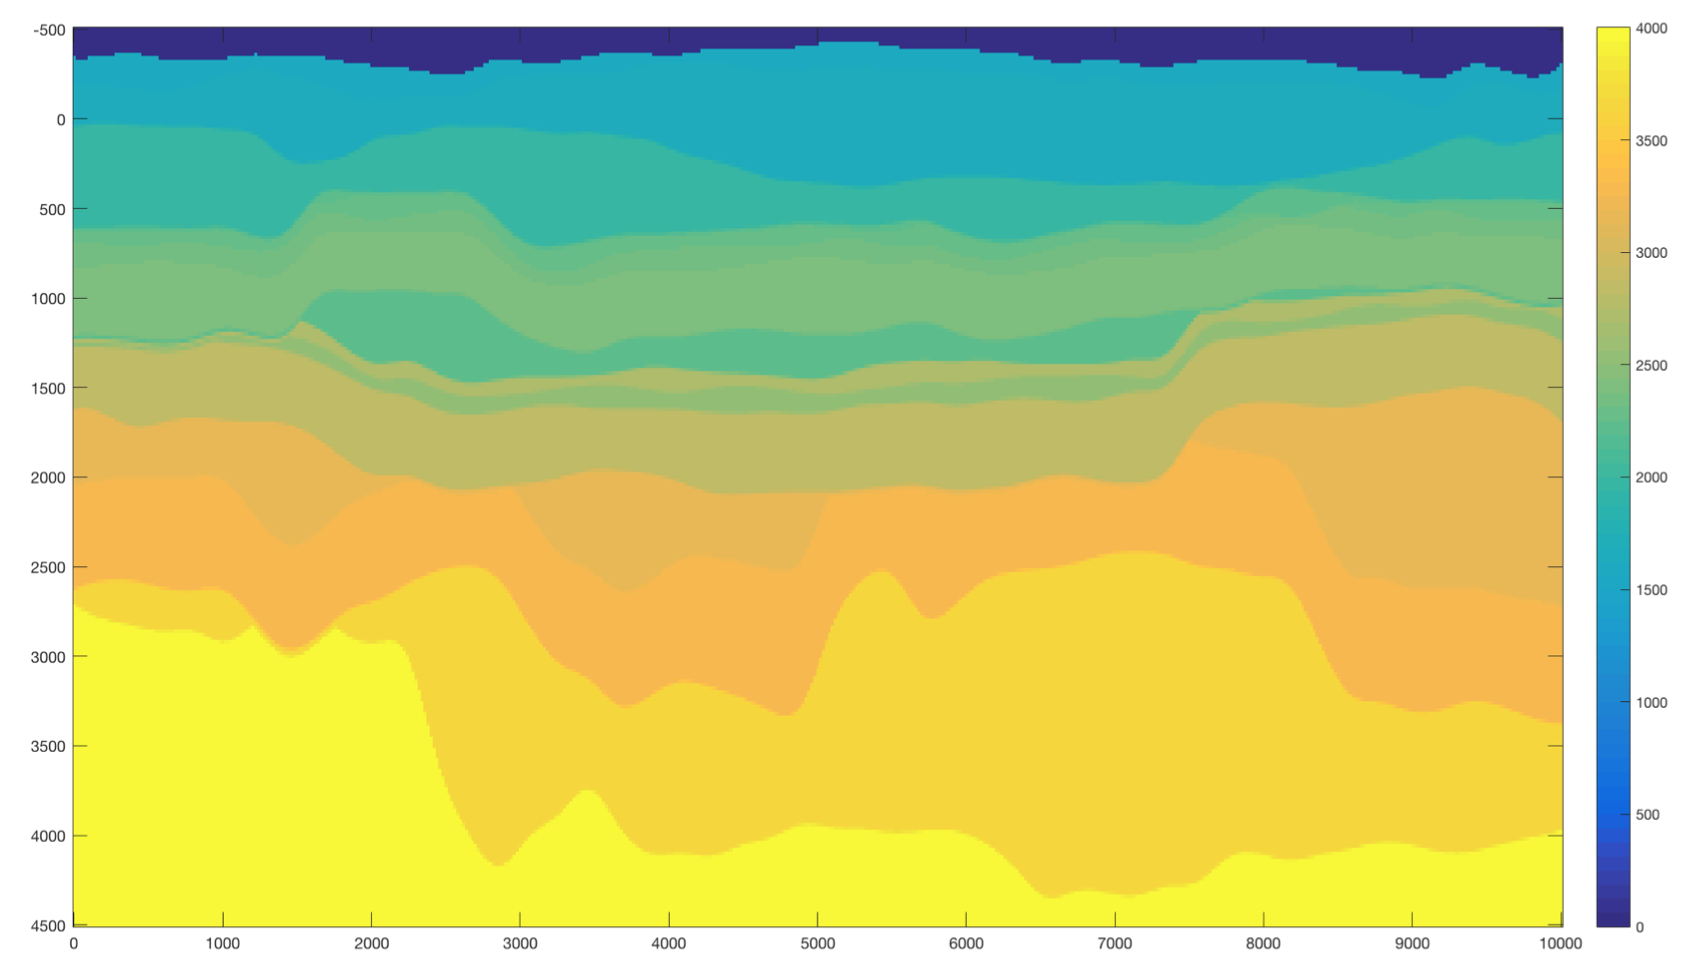
\includegraphics[width=0.8\textwidth]{images/velocity_field.png}
    \caption{One slice of the $250\times501\times501$ cube. In the slice we can distinguish between the different layers.}
    \label{fig:slice1}
\end{figure}

This script is to us as a mathematical model $v_{p}(x,y,z) = \mathcal{M}(v_{p})$ that receive $v_{p}$ as an input variable and generate a $v_{p}(x,y,z)$ as an output. In the benchmark the values of $v_{p}$ are fixed (Table \ref{tab:valuesOfVp}), so we cannot use it as is. We need to take the input, $v_{p}(m/s)$  in this case, as a random variable. To achieve this, we designate a \textit{PDFs} to each $v_{p}$ for each layer as shown in Table \ref{tab:PDFsOfVp}.

\begin{table}
\begin{center}
    \begin{tabular}{|l|l|l|}
    \hline
    \textbf{Layer} & \textbf{PDF Family}                & \textbf{Parameters}           \\ \hline
    1     & Gaussian & [1619, 711.2] \\ \hline
    2     & Gaussian & [3368, 711.2]               \\ \hline
    3     & Gaussian & [8839, 711.2]               \\ \hline
    4     & Gaussian & [7698, 301.5]               \\ \hline
    5     & Lognormal   & [7723, 294.7]               \\ \hline
    6     & Lognormal   & [7733, 292.2]               \\ \hline
    7     & Lognormal   & [7658, 312.1]               \\ \hline
    8     & Lognormal   & [3687, 368.7]               \\ \hline
    9     & Exponential & [3949, 394.9]             \\ \hline
    10   & Exponential & [5983, 711.2]               \\ \hline
    11   & Exponential & [3520, 352.0]              \\ \hline
    12   & Exponential & [3155, 315.5]              \\ \hline
    13   & Uniform     & [2541, 396.4]              \\ \hline
    14   & Uniform     & [2931, 435.3]              \\ \hline
    15   & Uniform     & [2948, 437.0]             \\ \hline
    16   & Uniform     & [3289, 471.1]              \\ \hline
    \end{tabular}
    \caption {PDFs and its parameters used to sampling the $v_{p}$, to generate n velocity models.}
    \label{tab:PDFsOfVp}
    \end{center}
\end{table}

Now, using a Monte Carlo method we can sampling the input variable $v_{p}$ and run as many simulations as we want using the model $v_{p}(x,y,z) = \mathcal{M}(v_{p})$, to posteriorly analyze the uncertainty in the output $v_{p}(x,y,z)$. An example of 1000 samplings of $v_{p}$ is shown in Figure \ref{fig:vp_1000_realizations}. Is clear that this is a not a real problem as a benchmark was not conceived as an uncertainty problem, but the datasets generated here are useful for our purposes.

\begin{figure}[ht]
    \centering
    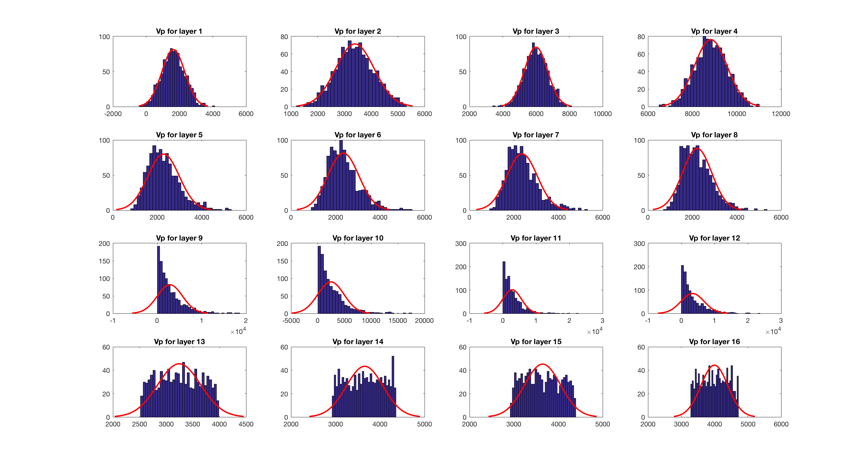
\includegraphics[width=0.8\textwidth]{images/vp_1000_realizations.png}
    \caption{Histograms of the 1000 samplings generated using Monte Carlo method and the PDFs reported in Table \ref{tab:PDFsOfVp}.}
    \label{fig:vp_1000_realizations}
\end{figure}

We generate three datasets, each one characterized by the dimensions $x \times y \times z$ of the cubes and the number of simulations. The datasets are name dataset1, dataset2 and dataset3, and its characteristics are summarized in Table \ref{tab:datasets}.

\begin{table}[H]
\centering
\begin{tabular}{c|c|c|c|}
\cline{2-4}
                               & dimensions                & simulations & size   \\ \hline
\multicolumn{1}{|c|}{dataset1} & $250\times501\times501$   & 1000        & 235 GB \\ \hline
\multicolumn{1}{|c|}{dataset2} & $501\times1001\times1001$ & 1000        & 1.9 TB \\ \hline
\multicolumn{1}{|c|}{dataset3} & $250\times501\times501$   & 10000       & 2.4 TB \\ \hline
\end{tabular}
\caption{Dimensions, number of simulations and size of the three datasets used to evaluate the computational cost of the \textbf{PDF} on a \textbf{LSSTM}.}
\label{tab:datasets}
\end{table}

\section{Architecture for Computing PDFs in Spark}\label{sec:spark_architecture}
We use two cluster testbeds, each with NFS, HDFS and Spark deployed. The first one, which we call LNCC cluster, is a cluster located at LNCC with 6 nodes, each having 32 CPU cores and 94 GB memory. The second one is a cluster of Grid5000, which we call G5k cluster, with 64 nodes, each having 16 CPU cores and 131 GB of RAM storage.

\section{Experimental Evaluation}\label{sec:experiments}

\section{Summary}\label{sec:summary}
The main conclusion of this Chapter is that compute a \textbf{PDF} on each spatio-temporal location is a computationally intensive task. The computational time can be reduced with 
